\documentclass[a4paper, 10pt]{report} % perhaps book?
\usepackage{graphicx}
\usepackage{url}
\usepackage{amsmath}
\begin{document}
\title{Mufasa Intro}
\author{Merlijn Wajer \and Raymond van Veneti\"{e}}
\maketitle
\tableofcontents

\chapter{Introduction}

\emph{This is the official Mufasa Documentation.
The main purpose of this document is to provide a clear view on Mufasa's 
interal structure. This guide is aimed at developers and other persons
interested in project Mufasa.}

\section{What is Mufasa?}

Mufasa is a project that aims to create the Mufasa Macro Library (MML).
As a side project, the project also tries to create a simple but effective
user interface to the Mufasa Macro Library. This is achieved with the
Pascal interpreter PascalScript\footnote{
\url{http://www.remobjects.com/ps.aspx}} combined with a wrapper for the MML.

Mufasa is:
\begin{itemize}
	\item Object Oriented. Since OOP also increases the abstraction of
		  certain tasks/parts, the code is much easier to maintain and
		  comprehend.
	\item Free Software, as in, Freedom.
			\footnote{http://www.gnu.org/licenses/gpl.txt}
	\item Cross platform. Currently the supported platforms are Linux 
		  (32 and 64 bit) and Windows (32 and 64 bit).
		  Mac support is planned; but currently halted due to lack of a
		  Mac computer.\footnote{Virtual Machines are an option;
		  but currently Darwin is not supported on Virtualbox.}
	\item A community project; the SRL community\footnote{
			\url{http://www.villavu.com}}
		  is widely known for it's maturity and open-mindedness.
	\item Mufasa is actively maintained. It also has a bugtracker,
		  a wiki, and a forum.
	\item A great project to participate in if you want to sharpen your
		  coding skills.
		  \pagebreak
	\item A project that has lots of possibilities. Among these are
		  running a "macro" service that clients can use to 
		  connect to. Possibly even remote; which means it would
		  also be possible to create a remote-client for the phone.
		  This service thread would be multithreaded, and support
		  running multiple scripts from one computer. \\
		  Now, these are only ideas, but they aren't fully impractical,
		  and it is possible to make this, with the right effort. \\
	\item Open minded. We appreciate your help, ideas and critisism!
	\item Well documented. Well... At least we are aiming towards being
		  well documented, but there is still some work left.
\end{itemize}

\pagebreak

\subsection{Mufasa Macro Library}

The MML's main features are:
\begin{itemize}
	\item Mouse control.
	\item Keyboard control.
	\item Screen capturing and analyzing.
	\item Providing several methods to analyzing the screen; among these
		  are DTM's and Bitmaps.
	\item API's to open files and web pages.
\end{itemize}

\subsection{Mufasa GUI}

As mentioned in the introduction, the Mufasa GUI uses Pascal Script as 
interpreter. \\ 

A non-OOP MML wrapper has been created only for the purpose
of exporting MML functionality to Pascal Script. 
This allows the user to use MML functions in their so called `Scripts'. \\
A more detailed specification will be given once we have explored the MML.

\chapter{The Mufasa Macro Library and it's Core Classes}

The Mufasa Library consists out of one class that combines all the other
classes, the \textbf{Client} class.

\section{The Client Class}

The \textbf{Client} class is the main Class, and is designed 
to run seperately from the User Interface.
The Client class is mainly designed to be a container for other classes.
If one wants to use the MML as a whole, they will only need the use 
the Client class.

\begin{figure}[ht]
	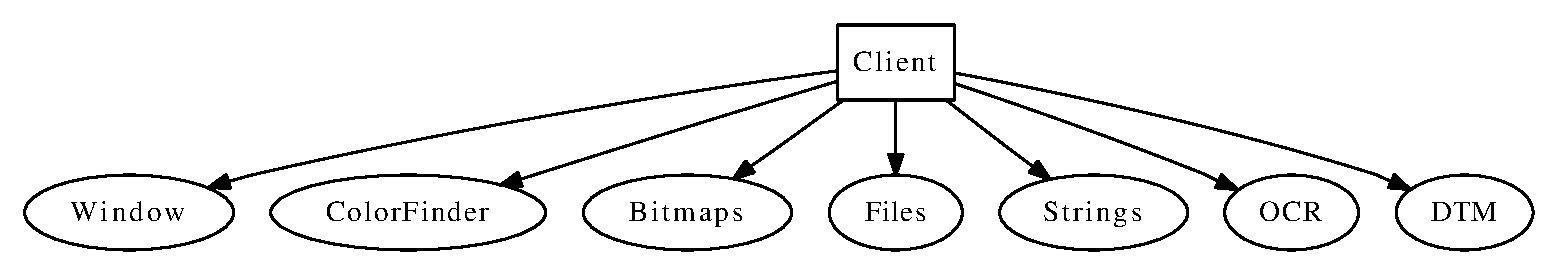
\includegraphics[scale=0.4]{Pics/Client_Classes}
	\caption{Classes that the Client contains.}
\end{figure}

\pagebreak

\section{The Window Class}

The \textbf{Window} class manages the core functionality for retreiving Window data,
such as the actual pixel data and the position and dimension of a window. \\

The Window class' main purpose is to form a cross platform class to retrieve
window information; no other class than the Window class should have to do
any platform-specific function calls to retreive window data; this is all
abstracted by the Window class.\footnote{This implements the so-called 
encapsulation of functionality.} \\

The Window class:

\begin{figure}[ht]
	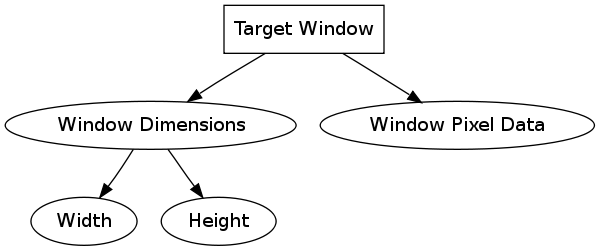
\includegraphics[scale=0.4]{Pics/Window}
	\caption{Simplified structure of the Window class}
\end{figure}

Figure 2.2 is ofcourse a highly simplified representation of the Window class;
the real class implements several other features. Among those are copying
(parts) of a window to a bitmap, methods to set a window as target, and
a feature that allows the user to ``Lock'' the Windows' current data in
Mufasa-maintained memory. \\

\subsection{Quick overview of functions}

\begin{itemize}
	\item ReturnData
	\item FreeReturnedData
	\item GetDimensions
	\item SetTargetWindow
	\item SetTargetIntArray
	\item SetTargetXWindow
	\item GetPixel
\end{itemize}

Together, these functions form the core of the window management.
However; to fake user input, a programmer also needs the ability to 
manipulate user input. Which brings us to the next MML Core class.

\subsection{Freeze}

The Window class also contains a feature called `Freeze'.
Freeze allows one to save the current Client's Window data.
All further methods that use the Client's Window data now use the saved
data, until `UnFreeze' is called. \\

This feature was easy to implement since we only had to modify the
`ReturnData' method. If used wisely, this can speed up your program
a lot, depending on the client size. It makes FindColorsTolerance about
6 times faster on my system.

\section{The Input Class}

The \textbf{Input} Class is the class that takes care of all the input. \\
As one can see in Figure 4, MML aims to support both Silent and non Silent 
Input. Since the Input heavily differs per operating system, 
the Input class should have a general way of sending keys,
possibly at the expense of losing some functionality.

\subsection{Silent Input}

So what is Silent Input?
We\footnote{The Designers and Developers of Mufasa} define Silent Input as
methods to manipulate the user's mouse and keyboard, without visually using
them. So what does this mean? \\

This basically means that you will still be able to use your mouse while
MML is performing mouse operations on your targetted window/client.

However, silent input is very hard to implement, and often hardly supported
by host operating systems. Often silent mouse or keyboard input is simply 
ignored. So in general it is advised to stick to non silent input.


\begin{figure}[ht]
	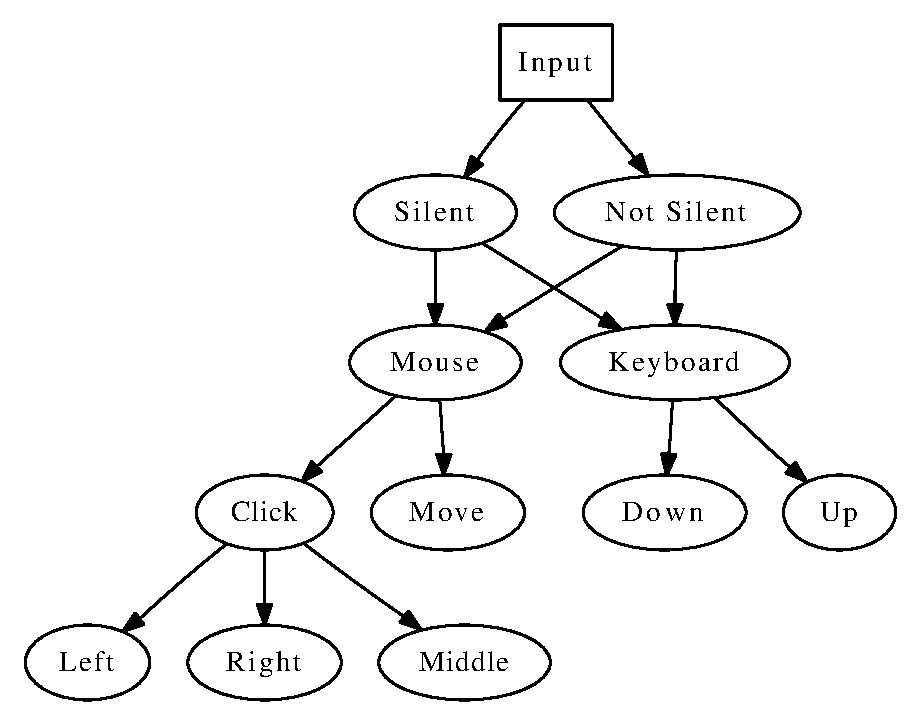
\includegraphics[scale=0.4]{Pics/Input_Diag}
	\caption{Input Functionality.}
\end{figure}

\section{The Colour Conversions Include}

The \textbf{Colour Conversions} unit contains pascal code to quickly convert
one colour type to another. It also adds support for comparing colours.
The reason this is not a class, is because constantly dereferencing a class
to call a single\footnote{Small} function won't do the speed of a program any 
good. There also wasn't really a need for a class,
since none of these functions need to be initialized in any way.

\section{The Colour Class}

The colour class is a Class that does all the colour identfying and locating
work. (A function like FindColor does this)
The colour class uses the Colour Convertions unit for several of it's
functions.

A FindColor-derivative function in Mufasa exists generally out of the following
steps:
\begin{itemize}
	\item Retrieve Client Data.
	\item Loop over the data, possibly with a special (spiral) algorithm.
	\item Check the current pixel data against another colour, possibly 
		  with tolerance.
	\item Free the Client Data.
	\item Return found point(s).
\end{itemize}

\begin{figure}[ht]
    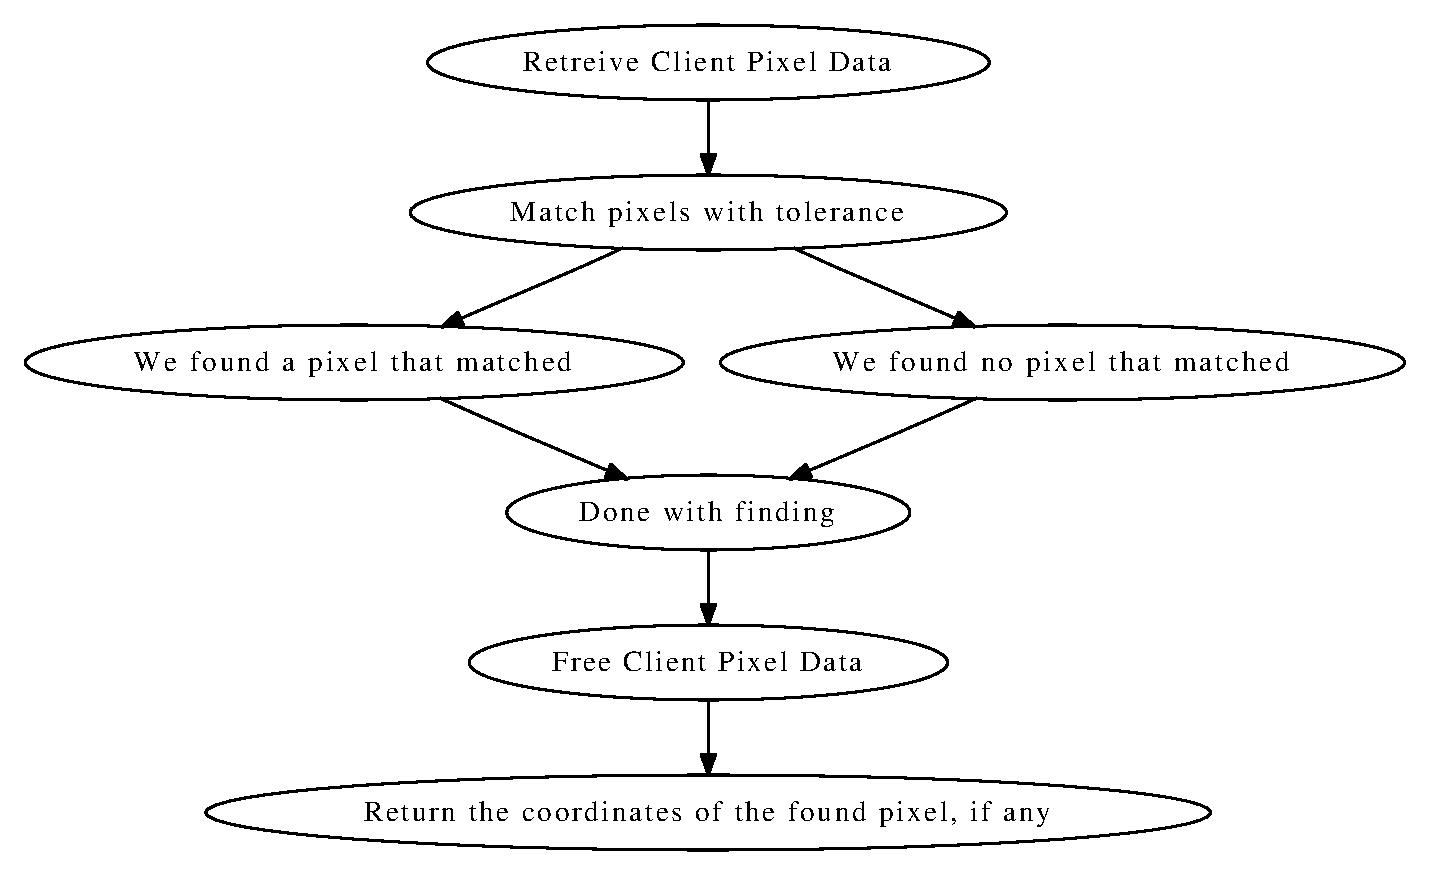
\includegraphics[scale=0.4]{Pics/FindColor}
    \caption{A basic find colour.}
\end{figure}

\section{DTMs and the DTM Class}

DTM is shorthand for Deformable Template Model. \\

\emph{``DTM'' is the term used in SCAR. If it is actually a Deformable Template
Model is definately debateable; but for now we will stick to ``DTM''.} \\

A DTM is in my view just a relatively simple way of defining a relationship
between several points. Each of these points have a relative offset to each
other, and may different in colour, tolerance, area size and shape.
A DTM generally consists out of one \textbf{Main Point}, and several
\textbf{Sub Points}
The structure of a DTM looks like this:

\begin{figure}[ht]
    \includegraphics[scale=0.4]{Pics/DTM}
    \caption{Structure of a DTM.}
\end{figure}

Where each point in a DTM has a colour, tolerance, area size and area shape
entity. The main point's ``point'' is typically $ (0, 0) $, and all the
sub point points are arelative to the main point.

\subsection{DTM Structure in MML}

\begin{verbatim}
  pDTM = record
    l: Integer;
    p: TPointArray;
    c, t, asz, ash: TIntegerArray;
    bp: Array Of Boolean;
    n: String;
  end;                                           
\end{verbatim}

\subsection{Example of a simple DTM}
If one was to create his own DTM, he\footnote{Or she, but we will denote he
and she as ``he'' in this article.} would first have to think of a usefull DTM
structure.

Say:
$$ MainPoint = (123, 456)  $$
$$ SubPoint_1 = (122, 460) $$
$$ SubPoint_2 = (120, 450) $$

Then we could create the following pDTM structure:

\begin{verbatim}
	// Give dtm.p a length of three.
	// Mainpoint
	dtm.p[0] = Point(123, 456);

	// Subpoints
	dtm.p[1] = Point(122, 460)
	dtm.p[2] = Point(120, 450)
\end{verbatim}

Note that we do not include other variables, such as colour, tolerance, area
size and area shape; they are of no importance in this example.

However, this code is not very clear about the DTM's points.
Better would be to write:

\begin{verbatim}
    // Give dtm.p a length of three.
    // Mainpoint
    dtm.p[0] = Point(0, 0);

    // Subpoints
    dtm.p[1] = Point(-1, 4)  // 122 - 123 = -1, 460 - 456 = 4
    dtm.p[2] = Point(-3, -6) // 120 - 123 = -3, 450 - 456 = -6
\end{verbatim}

As you can see it is perfectly valid to use negative points.

\subsection{Colour and Tolerance}

The colour value of a point in a DTM is just a RGB integer value.
Black = 0, Red = 255, White = 16777215, et cetera.

The value tolerance decides if a colour is similar enough to the given
colour; if this is the case, we say that the colours \textbf{matched}.

With no Area Size and Area Shape specified\footnote{Read: with Area
Size = 0 and Area Shape = Rectangle} we say that a DTM matches if for each
point in the DTM, the colour at the relative point matches the colour in dtm
with the given tolerance.

$$ \forall p \in P, \forall t \in Tol, \forall c \in Col : T(C(p), c) \leq t $$

With C() defining the colour at the given point, and T() defining the tolerance
between the two given colours.

\subsection{Area Size and Shape}

Area Size and Shape add that nifty extra functionality to DTM's.
\textbf{Area Size} defines the area that should all match the colour
with the given tolerance. \\
\textbf{Area Shape} is currently not implemented, mainly because
we haven't found a good use for area shapes.

%The \textbf{Area Shape} defines the Shape of the Area Size.
%Currently, the following shapes are supported:
%\begin{itemize}
%	\item Rectangle
%	\item Cross
%	\item DiagonalCross
%	\item Circle
%	\item Triangle\footnote{Not fully implemented yet.}
%\end{itemize}

\subsection{Loading a DTM from a string}

It is also possible to load a DTM from a ``zipped'' string.
The details of the algorithm will not be explained here.\footnote{Take
a look at the code in dtm.pas}

\subsection{pDTM and TDTM}

One may know DTM's as a different type:

\begin{verbatim}
  TDTMPointDef = record
    x, y, Color, Tolerance, AreaSize, AreaShape: integer;
  end;

  TDTMPointDefArray = Array Of TDTMPointDef;

  TDTM = record
    MainPoint: TDTMPointDef;
    SubPoints: TDTMPointDefArray;
  end;            
\end{verbatim}

The MML provides the two functions \textbf{pDTMtoTDTM} and \textbf{TDTMtopDTM} to
directly convert between the two types.

\subsection{Main Point and AreaSize / Shape}

The main point's area size and shape are not used in the current
implementation. It wouldn't be that hard to add them, however.

%\subsection{DTM algorithm}


\section{Bitmaps and the Bitmaps Class}

\subsection{Introduction to Mufasa Bitmaps}
To understand how the bitmaps in MML work, we will first make a 
distinguishment between two different objects; the Bitmap Manager and the 
Bitmap itself. The bitmap manager contains and manages a pool of bitmaps.


\subsection{The Bitmap}

Mufasa has it's own implementation of a Bitmap.
A bitmap is basically just a piece of bytes, ordered in a certain fashion.
We have extended this concept to a full blown Bitmap class: ``TMufasaBitmap''.
The data per pixel consists out of 32 bits\footnote{4 bytes}, and is 
``stored'' in the variable ``FData'', of the type ``TRGB32''.
FData is a pointer to the data in memory.
The advantage of a 32 bit structure to a 24 bits structure, consists mainly
of the fact that 32 bits are more easily accessed that 24 bits. 32 bits are
aligned in such a fashion that they are easily accessed, and translated to
other formats\footnote{Or just ``Colours''}.

\subsection{Example of usage}
As you can directly access the rawdata, bitmap functions will be fast and 
easy to use. Since the data is stored as an array you need to do convert your
coordinate into a array-index using the following transformation:
$$ \{\forall (x, y) \in Points,\ \forall\ i \in Index: i = (x * w) + x \} $$

With ``w'' as the Bitmap width.

For example we want to change pixel (5,20) to clWhite and our bitmaps
width = 50:
\begin{verbatim}
Bitmap.FData[20 * 50 + 5].r := 255;
Bitmap.FData[20 * 50 + 5].g := 255;
Bitmap.FData[20 * 50 + 5].b := 255;
\end{verbatim}

\subsection{Naming a bitmap}
You can also name a bitmap by setting the BmpName property.
This may come in handy when working with multiple bitmaps.

\section{Finder class}
The finder class contains all the methods that are used to ``identify''
pixels\footnote{Also contains methods for bitmaps on bitmaps, dtms, etc} 
and more on other bitmaps; or just on a window.

\section{Notes on the previously mentioned classes}


\section{More On The Core Classes}

The previously mentioned MML classes are considered to be the absolute core 
`of the library. (Although one could argue that even the Colour class isn't
part of the core classes.)

With these classes most functions that Mufasa will contain can be created.
If you can make FindColor, you can make FindColorsSpiralTolerance, 
they don't really differ a lot. The same goes for DTM's, OCR and Bitmaps.
Mouse and keyboard functions will be done with the Input class.

The MML contains more classes, and they will mainly utilize the previous
mentioned classes. It is essential to understand the Classes architecture
to fully understand Mufasa. Before work on other classes will be done,
the core classes must be finished and stable.

A good rule of thumb is the following: any units that make extensive use of
Compiler Directives, are considered a core unit.

\end{document}
